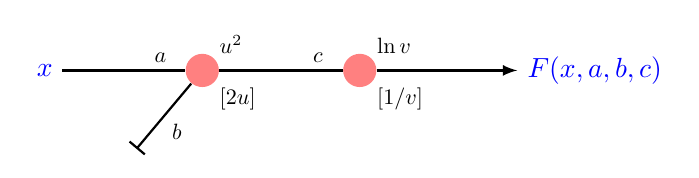
\begin{tikzpicture}
\def\layersep{2cm}
\tikzstyle{neuron}=[circle,fill=red!50,minimum size=12pt,inner sep=0pt]

% Entree
\node[blue] (E) at (-\layersep,0) {$x$};

% Neurone F
\node[neuron] (F) at (0,0) {};
\node[above right=0.8ex,scale=0.8] at (F) {$u^2$};
\node[below right=0.8ex,scale=0.8] at (F) {$[2u]$};
 \path[thick] (E) edge node[pos=0.8,above,scale=0.8]{$a$} (F);
 \draw[-|,thick] (F) to node[midway,below right,scale=0.8]{$b$} ++ (-130:1.3);

% Neurone G
\node[neuron] (G) at (\layersep,0) {};
\node[above right=0.8ex,scale=0.8] at (G) {$\ln v$};
\node[below right=0.8ex,scale=0.8] at (G) {$[1/v]$};
 \path[thick] (F) edge node[pos=0.8,above,scale=0.8]{$c$} (G);


\draw[->,>=latex,thick] (G)-- ++(2,0) node[right,blue]{$F(x,a,b,c)$};

\end{tikzpicture}  